%%This is a very basic article template.
%%There is just one section and two subsections.
%\documentclass[12pt,oneside,a4paper,doublespacing]{article} % for submission
\documentclass[11pt,oneside,a4paper]{article} % for sharing

\usepackage{appendix}
\usepackage{amsmath}
\usepackage{caption}
\usepackage{placeins}
\usepackage{graphicx}
\usepackage{subcaption}
%\usepackage{subfig}
\usepackage{longtable}
\usepackage{setspace}
%\usepackage{tikz}
\usepackage{booktabs}
\usepackage{tabularx}
\usepackage{xcolor,colortbl}
\usepackage{chngpage}
%\usepackage[active,tightpage]{preview}
\usepackage{natbib}
\bibpunct{(}{)}{,}{a}{}{;} 
\usepackage{url}
\usepackage{nth}
\usepackage{authblk}
\usepackage[most]{tcolorbox}
%\usepackage{hyperref}
%\usepackage{color}
%\usepackage{fontspec}
%\usepackage{pdfsync}
\usepackage[normalem]{ulem}
\usepackage{amsfonts}
\renewcommand{\listtablename}{List of Appendix Tables}
\newcolumntype{C}[1]{>{\centering\let\newline\\\arraybackslash\hspace{0pt}}m{#1}}
\newcolumntype{L}[1]{>{\raggedright\let\newline\\\arraybackslash\hspace{0pt}}m{#1}}
% working on this need to concatenate file name based on sex and variable name
%\newcommand\Cell[1]{{\raisebox{-0.05in}{\includegraphics[height=.2in,width=.2in]{Figures/ColorCodes/\expandafter#1}}}}  

%%%%%%%%%%%%%%%%%%%%%%%%%%%%%%%%%%%%%%%%%%%%%%%%%%%%%%%%%%%%%%%%%%%%%%%%%%%%%
% setting color to letters affects spacing. Here's a hack I found here:
% http://tex.stackexchange.com/questions/212736/change-letter-colour-without-losing-letter-spacing
%\DeclareRobustCommand{\spacedallcaps}[1]{\MakeUppercase{\textsc{#1}}} % all
% caps with better spacing

%\colorlet{RED}{red}
%\colorlet{BLUE}{b}
\colorlet{rd}{red}
\colorlet{bl}{blue}

%%%%%%%%%%%%%%%%%%%%%%%%%%%%%%%%%%%%%%%%%%%%%%%%%%%%%%%%%%%%%%%%%%%%%%%%%%%%%%

\newcommand\ackn[1]{%
  \begingroup
  \renewcommand\thefootnote{}\footnote{#1}%
  \addtocounter{footnote}{-1}%
  \endgroup
}
\newcommand\vt[1]{\textcolor{rd}{#1}}
\newcommand\eg[1]{\textcolor{bl}{#1}}

\newcommand\tg[1]{\includegraphics[scale=.5]{Figures/triadtable/triad#1.pdf}}
\newcommand\tgh[1]{\raisebox{-.25\height}{\includegraphics[scale=.3]{Figures/triadtable/triad#1.pdf}}}

\defcitealias{HMD}{HMD}

% junk for longtable caption
\AtBeginEnvironment{longtable}{\linespread{1}\selectfont}
\setlength{\LTcapwidth}{\linewidth}

%%%%%%%%%%%%%%%%%%%%%%%%%%%%%%%
\begin{document}

\title{A unified model of demographic time}

\author[1]{Tim Riffe\thanks{triffe@demog.berkeley.edu}}
\author[2,3]{Jonas Sch{\"o}ley}
\author[2,3]{Francisco Villavicencio}
\affil[1]{Max Planck Institute for Demographic Research}
\affil[2]{University of Southern Denmark}
\affil[3]{Max-Planck Odense Center on the Biodemography of Aging}

%\author{[Authors]}

\maketitle

\begin{abstract}
We describe a three-dimensional model that relates six different measures of
lifespans and time. The six measures of demographic time considered are
chronological age, thanatological age, lifespan, year of birth, year of death,
and period. Two versions of the model are described: a relatively intuitive
extension of the right-angled Lexis diagram, and an isotropic extension based on
the regular tetrahedron. \ackn{The work reported in this manuscript was begun by
the first author while at the Department of Demography at the University of
California, Berkeley, and was supported by the U.S.
National Institute On Aging of the National Institutes of Health under award
numbers R01-AG011552 and R01-AG040245. The content is solely the responsibility of the authors and does not necessarily represent the official views of the funding agencies.}
\end{abstract}
%\sout{so-called} \textbf{well-known?} 
The Lexis diagram relates the chronological age (A), period (P),
and birth cohort (C) measures of demographic time, APC, but it does not account
for remaining years of life (thanatological age), and other related time
indices.
The thanatological counterpart to APC is an identity between thanatological
age (T), period (P), and death cohort (D), TPD. A third
identity exists between chronological age (A), thanatological age (T), and lifespan (L), ATL, and a fourth between year of birth (C), year of death (D) and lifespan (L), CDL.
Each of these four identities may be sufficiently described by any
two of its consituent indices, making the third index redundant. Each of these
four identities also lacks a major dimension of time. The ATL identity
lacks calendar time, the CDL identity is ageless, APC lacks an endpoint in time,
and TPD lacks a starting point in time. We refer to these four identities
as the triad identities.

To our knowledge, the only triad identity that has received serious
treatment at the time of this writing is the APC identity. Different
aspects of the APC identity have been discussed since at least 1868
\citep{knapp1868ermittlung}, and discussion remains lively today. Here it is our
objective to relate the six major indices of time in a geometric identity, in
much the same spirit as the work on APC relationships done between the late
1860s and mid 1880s.\footnote{See e.g., \citet{keiding2011age} for an overview of that literature.} 

This paper provides a bottom-up description of the model, building from familar
components to the full relationship. We begin by defining some terms used
throughout the manuscript. We then explore all combinations of two time
measures, the dyadic relationships, followed by the four triad identities, and
finally the hexad identity. At the price of some redundancy, we give a systematic topological overview of the
different elements of demographic time. 

\section*{Definitions}
\subsection{Technical terminology}
We attempt to adhere to a rigorous terminology in this paper. The following list
describes some of the more important terms we use.
\begin{description}
\item[Time measures] are any of the six demographic perspectives discussed that
can be used to index time: chronological age ($A$), period ($P$), birth cohort ($C$), thanatological
age ($T$, time-to-death), lifespan ($L$), and death cohort ($D$).
\item[Dyads, triads, and hexads] are any set of two, three, or six unique time
measures, respectively.
\item[A temporal plane] is any $(x,y)$-mapping of a dyad of time measures.
\item[A temporal space] is any $(x,y,z)$-mapping of a triad of time
measures that generates a 3-dimensional space.
%\item\sout{[Given measures] are any specified set of time measures.}
%\item\sout{[Derived measures] are any unspecified time measures that are implied by or
%derived from a given set.} 
%\item\sout{[An informative] set is a set of given measures that entails at
%least one derived measure.}
%\item\sout{[An uniformative] set is a set of given measures that does not entail any
%derived measures.}
\item[A triad identity] is a triad that is the union of an informative dyad and
its one derived time measure. For example, $A$ and $P$ form an informative dyad
from which $C$ can be derived.
\item[A hexad identity] is a unique combination of the six time measures.
\end{description}
Using this terminology, for example, we say that the ``Lexis'' measures
constitute a triad identity between chronological age, period, and birth cohort. Each dyad
combination of elements in this identity is informative, and can be mapped to a
temporal plane, the Lexis diagram. If we know that Mindel turned 50 on the
\nth{21} of May, 1963, then we also also can derive that she was born on the \nth{21} of
May, 1913. Any two pieces of information in this case will give the third, which
means that any dyad from this set is informative. Three other such triad
identities are also to found within the six measures of time we discuss.
\FloatBarrier

\subsection*{Time measures}
\FloatBarrier
This model description is conceived in absolute, linear, Newtonian time, and we
do not consider situating the model in any other perspective or model of time
itself.
This relationship is scalable to any time unit, but we decribe it in terms of
years, the dominant human time scale. We therefore speak of calendar time,
imagining the modern Gregorian calendar, though this is not necessary. The six
measures of time we consider are defined in Table~\ref{tab:sixdefs}, both in the
demographic sense we describe, as well as in a more general event history
interpretation.

\begin{table}
\centering
\caption{Definitions of the six time measures.}
\label{tab:sixdefs}
\begin{tabular}{lcll}
\hline 
\textbf{Time measure} & \textbf{Short} & \textbf{Demographic def.} &
\textbf{Event history def.}\\
\hline 
chronological age & A & Time since birth & Time since study entry \\
period & P & calendar time & calendar time \\
birth cohort & C & calendar time of birth & calendar time of study entry \\
thanatological age & T & time until death & time until event \\
death cohort & D & calendar time of death & calendar time of event \\
lifespan & L & duration of life & duration of exposure \\
\end{tabular}
\end{table}


The concepts of thanatological age and death cohorts are likely less familar to
readers than the other measures we consider. Thanatological age is sometimes
referred to in the literature as remaining years of life, or time-to-death
(TTD), but we prefer the term thanatological age, and to think of the concept of
age in general as marking a position on a lifeline with respect to one of its
endpoints.
Chronological age and thanatological age are in this way complementary. Thanatological age is
different from the notion of prospective age, used by
\citet{sanderson2007new}, since prospective age is a relative term that reflects
a comparison of expectancies. Prospective age scales chronological age by
comparing mortality schedules, but it is neither an expectancy nor a statement
of remaining years of life. Thanatological age is meaningful without much
justification; it is the measure we all want to know, the thing we approximate
with remaining life expectancy.

Cohorts in general associate individuals that share a characteristic. In
demography the grouping characteristic is often a combination of place and time, such as
the cohorts of young demographers passing through a particular graduate program.
In this instance already, we accomodate the notion of a cohort for both the
start and endpoints of the program, but we say e.g., ``the class of 2015''
instead of the ``graduating cohort of 2015'', in contrast to ``cohort 37'', the
\nth{37} class of entering students since the start of the program.
These concepts are analagous to the ideas of birth and death cohorts we use here, though we do not often refer to the
deaths of a given year as a death cohort. In the time preceding
death, the members of a given death cohort have much in common, despite
heterogeneity with respect to time of birth. If the reader accepts this premise,
then the abstract construct of a death cohort is also meaningful in
the way that the other measures are.

Much of the work of demography is directed at the study of lifespan. Lifespan is
synonymous both with longevity, chronological age at death, and thanatological
age at birth. One's ultimate completed lifespan is constant throughout life,
though we have no knowledge of it until death: It is assigned retrospectively.
Demographers have more often used lifespan or age-at-death as a measure of mortality, or similar, than as a measure on which to compare individuals. 

Treating lifespan,
death cohorts, and thanatological age as temporal structuring variables
enables new classes of comparisons, models of understanding, and discovery,
akin to those unlocked by breaking down demographic phenomena by chronological age,
period, and birth cohort. The following sections will, in this sense, provide an
exhaustive classification of the ways in which these six measures of time can be juxtaposed to such ends.
We begin with all sets of two time measures, the informative and uninformative
temporal dyads.

\FloatBarrier

\section*{Informative and uninformative dyads}

Any mapping of two time measures to a ($x,y$) coordinate
system constitutes a temporal plane. If the two time measures in question are
members of the same triad identity, the third member is called a derived
measure. For instance, if we take the dyad $AP$, $C$ is called the derived
measure, and we make this dyadic relationship explicit by writing $AP(C)$.
The temporal plane that corresponds to this informative dydad is the contemporary representation of the
Lexis diagram. The dyads $AC(P)$ and $CP(A)$ also belong to the Lexis identity, but imply different less-common rotations and projections of the Lexis
diagram. 15 dyads are possible from our set of six time measures, 11 of
which are informative, and four of which have no derived time measure, and are
therefore called uninformative. The 15 dyads are summarized in
Table~\ref{tab:dyads}.

\begin{center}
  \small
  \begin{longtable}{m{0.13\textwidth}m{0.37\textwidth}m{0.17\textwidth}m{0.17\textwidth}}
  \caption{The 15 temporal dyads, with corresponding translations to Euclidean
  and ternary representations in temporal planes.\protect\footnotemark} 
  \label{tab:dyads} \\
  %%%%%%%%%%%%%%%%%%%%%%%%%%%%%%%%%%%%%%%%%%%%%%%%%%%%%%%%%%%%%%%%%%%%%%%%%%%%%
  \multicolumn{4}{c}{\textsc{Variations of the Lexis Diagram}} \\
  \midrule
  %%%% AP
  $$\begin{aligned}
    &AP(C) \\
    &C = P - A
  \end{aligned}$$ &
  The $AP(C)$ temporal plane constitutes the classical Lexis diagram. &
  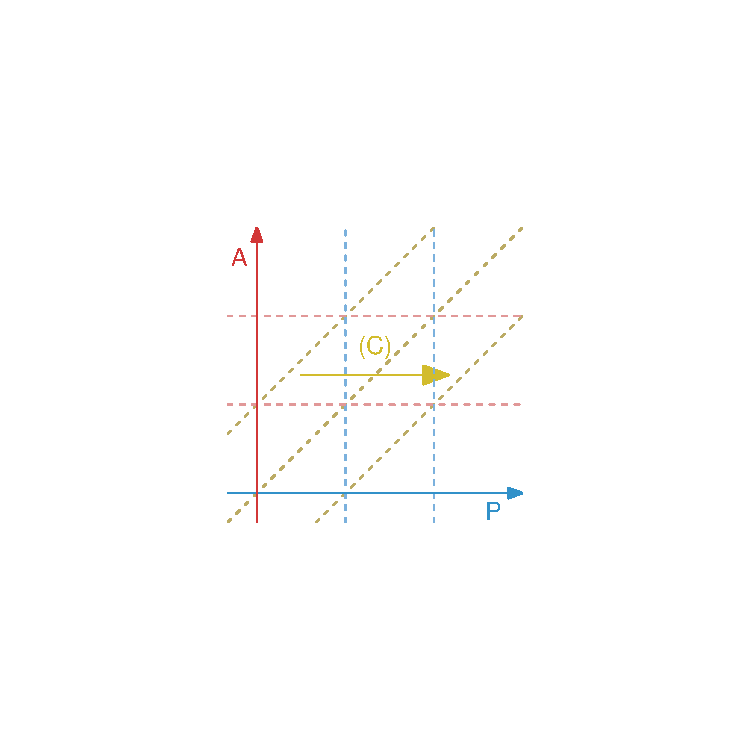
\includegraphics[width = \linewidth]{Figures/JonasTable/APc.pdf} &
  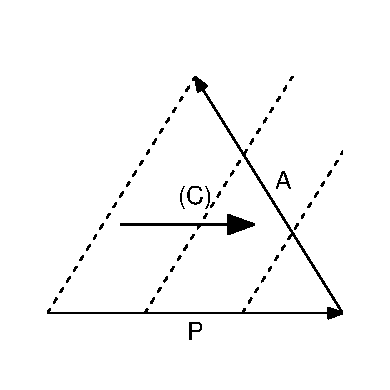
\includegraphics[width = \linewidth]{Figures/JonasTable/APc_iso.pdf}  \\
  \midrule
  %%%% AC
  $$\begin{aligned}
    &AC(P) \\
    &P = C + A
  \end{aligned}$$ &
  The $AC(P)$ temporal plane is equivalent to the Lexis diagram except that
  birth cohort is given and period is embedded instead of the other way round. & 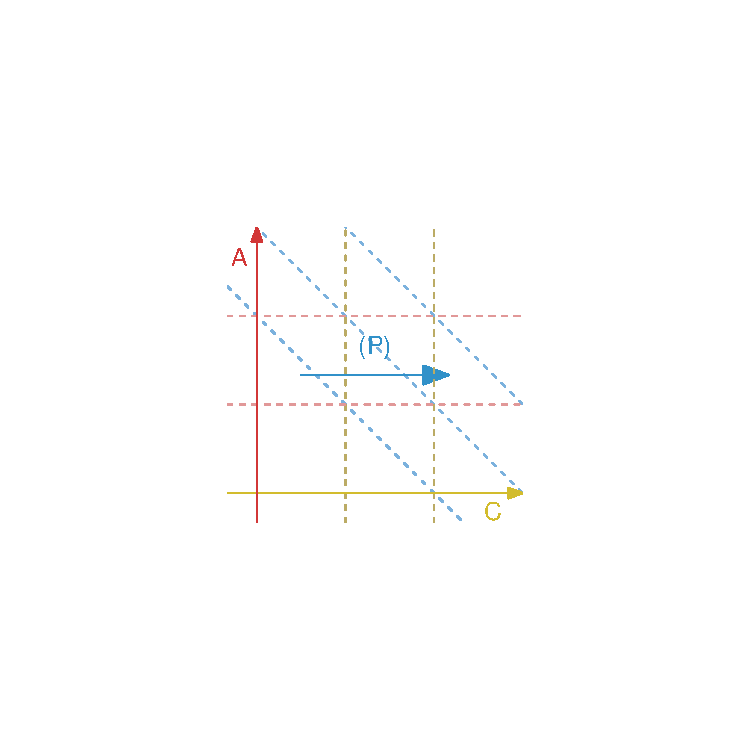
\includegraphics[width = \linewidth]{Figures/JonasTable/ACp.pdf} &
  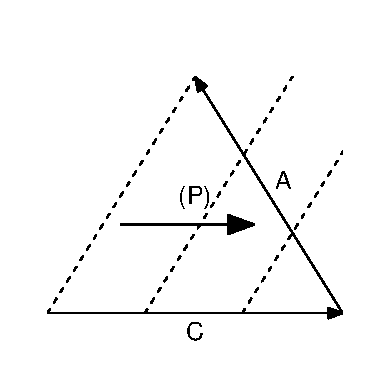
\includegraphics[width = \linewidth]{Figures/JonasTable/ACp_iso.pdf}  \\
  \midrule
  %%%% CP
  $$\begin{aligned}
    &CP(A) \\
    &A = P - C
  \end{aligned}$$ &
  The $CP(A)$ temporal plane is equivalent to the Lexis diagram except that birth cohort is given and age is embedded instead of the other way round. &
  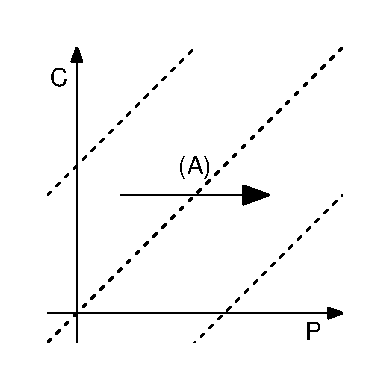
\includegraphics[width = \linewidth]{Figures/JonasTable/CPa.pdf} &
  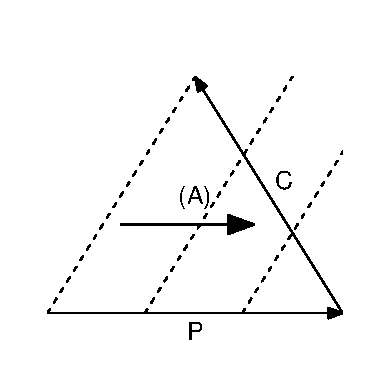
\includegraphics[width = \linewidth]{Figures/JonasTable/CPa_iso.pdf}  \\
  \midrule
  %%%%%%%%%%%%%%%%%%%%%%%%%%%%%%%%%%%%%%%%%%%%%%%%%%%%%%%%%%%%%%%%%%%%%%%%%%%%%
  \multicolumn{4}{c}{\textsc{2-D Combinations of Thanatological Scales}} \\
  \midrule
  %%%% LD
  $$\begin{aligned}
    &LD(C) \\
    &C = D - L
  \end{aligned}$$ &
  Margaret died in Dec., 1995 (D) with a completed lifespan of 96 (L), putting
  her birth year in 1900 (C). &
  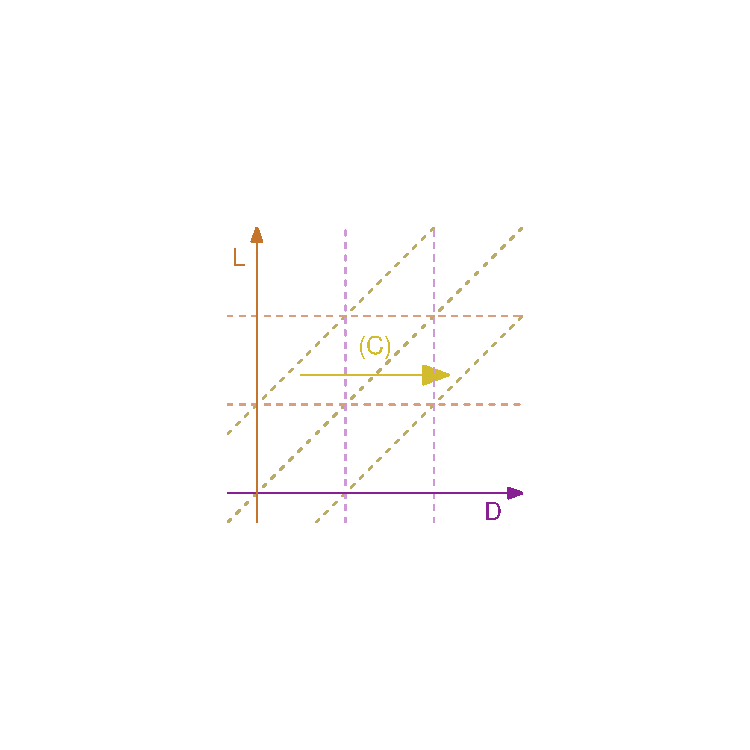
\includegraphics[width = \linewidth]{Figures/JonasTable/LDc.pdf} & 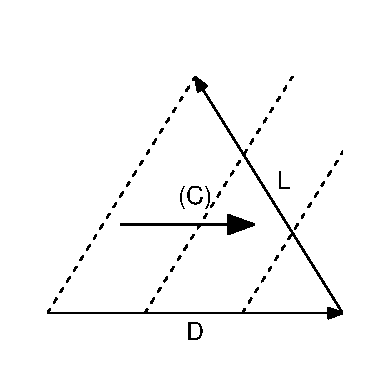
\includegraphics[width = \linewidth]{Figures/JonasTable/LDc_iso.pdf}  \\
  \midrule
  %%%% TL
  $$\begin{aligned}
    &TL(A) \\
    &A = L - T
  \end{aligned}$$ &
  Helen lived to the age of 86. When she had 20 years left she must have been
  66. & 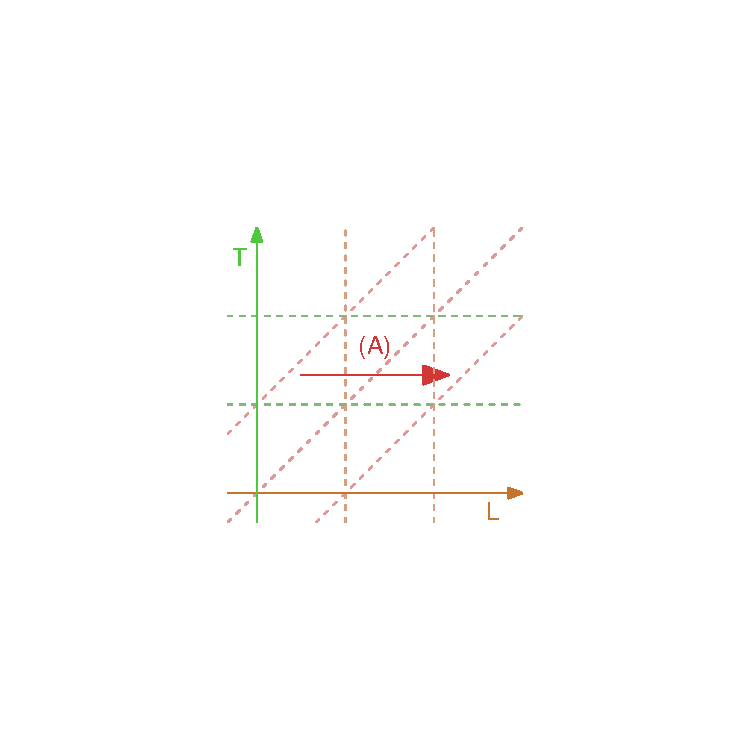
\includegraphics[width = \linewidth]{Figures/JonasTable/TLa.pdf} &
  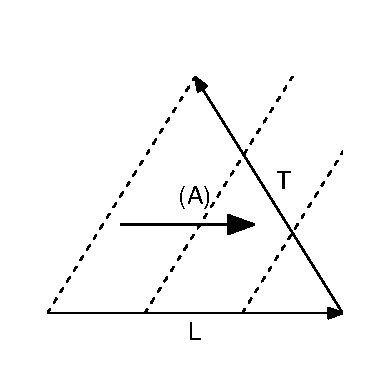
\includegraphics[width = \linewidth]{Figures/JonasTable/TLa_iso.pdf}  \\
  \midrule
  %%%% TD
  $$\begin{aligned}
    &TD(P) \\
    &P = D - T
  \end{aligned}$$ &
  Irene died in 1974. When she had 30 remaining years of life the year must
  have been 1944.& 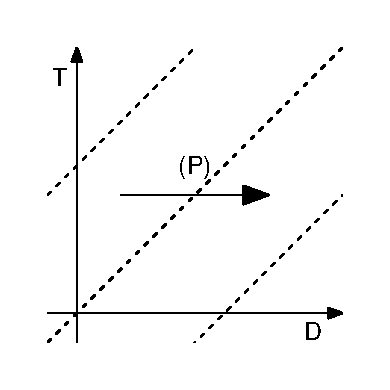
\includegraphics[width =
  \linewidth]{Figures/JonasTable/TDp.pdf} & 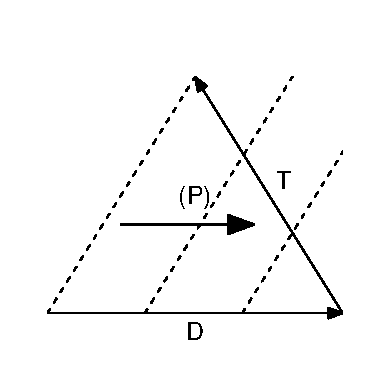
\includegraphics[width = \linewidth]{Figures/JonasTable/TDp_iso.pdf}  \\
  \midrule
  %%%%%%%%%%%%%%%%%%%%%%%%%%%%%%%%%%%%%%%%%%%%%%%%%%%%%%%%%%%%%%%%%%%%%%%%%%%%%
  \multicolumn{4}{c}{\textsc{2-D Combinations of Lexis Scales and Thanatological Scales}} \\
  \midrule
  %%%% AL
  $$\begin{aligned}
    &AL(T) \\
    &T = A - L
  \end{aligned}$$ & \footnotetext{The
  temporal planes are named after the two given time scales. The derived scale
  is appended in parentheses. Contrary to mathematical convention we name the ordinate scale first and the abscissa scale second. This is to be consistent with the established $APC$ and $ACP$ terms.}
  
  Tim is 34 years old (A) and will live to the age of 96 (L), leaving him 62
  years (T) to settle affairs.
  & 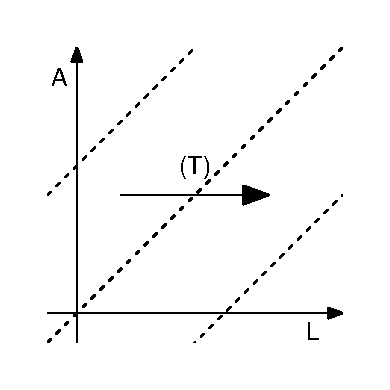
\includegraphics[width = \linewidth]{Figures/JonasTable/ALt.pdf} &
  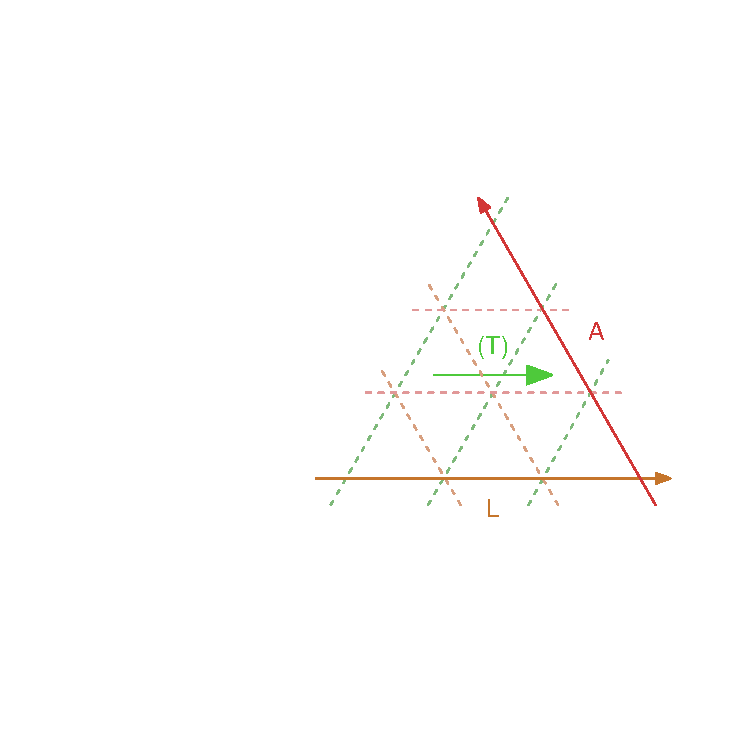
\includegraphics[width = \linewidth]{Figures/JonasTable/ALt_iso.pdf}  \\
  \midrule
  %%%% LP
  $LP(-)$ &
  The $LP$ plane is \emph{non-informative}. No additional dimensions can be derived knowing just lifespan and period. &
  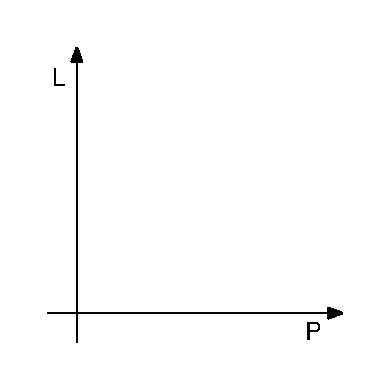
\includegraphics[width = \linewidth]{Figures/JonasTable/LP.pdf} &
  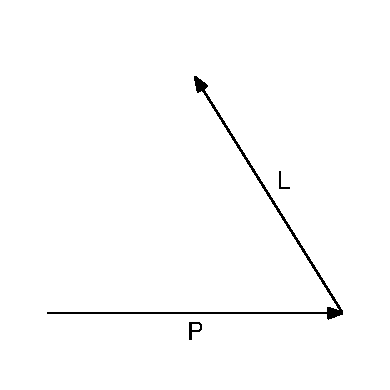
\includegraphics[width = \linewidth]{Figures/JonasTable/LP_iso.pdf}  \\
  \midrule
  %%%% PD
  $$\begin{aligned}
    &PD(T) \\
    &T = D - P
  \end{aligned}$$ &
  Mindel died in 1973 (D). In 1953 (P) she had 20 (T) years left to live. &
  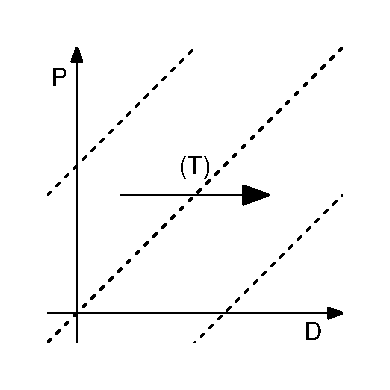
\includegraphics[width = \linewidth]{Figures/JonasTable/PDt.pdf} &
  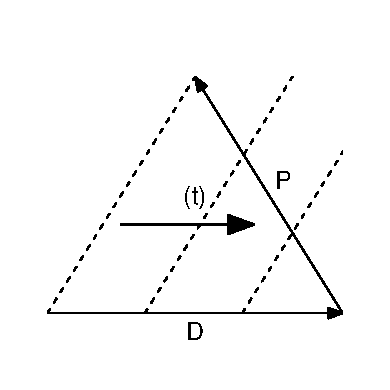
\includegraphics[width = \linewidth]{Figures/JonasTable/PDt_iso.pdf}  \\
  \midrule
  %%%% CD
  $$\begin{aligned}
    &CD(L) \\
    &L = D - C
  \end{aligned}$$ &
  Pascal was born in 1893 (C) and died in 1964 (D), implying a lifespan of 71
  (L), or so.
  & 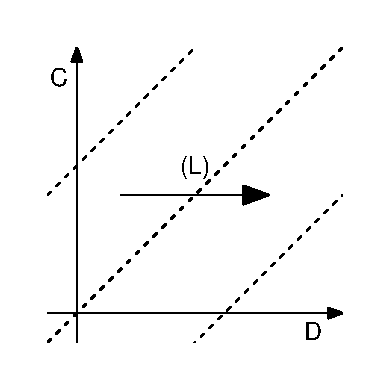
\includegraphics[width = \linewidth]{Figures/JonasTable/CDl.pdf} &
  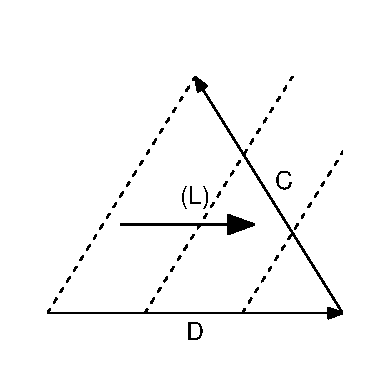
\includegraphics[width = \linewidth]{Figures/JonasTable/CDl_iso.pdf}  \\
  \midrule
  %%%% CT
  $CT(-)$ &
  The $CT$ plane is \emph{non-informative}. No additional dimensions can be derived knowing just cohort and thanatological age. &
  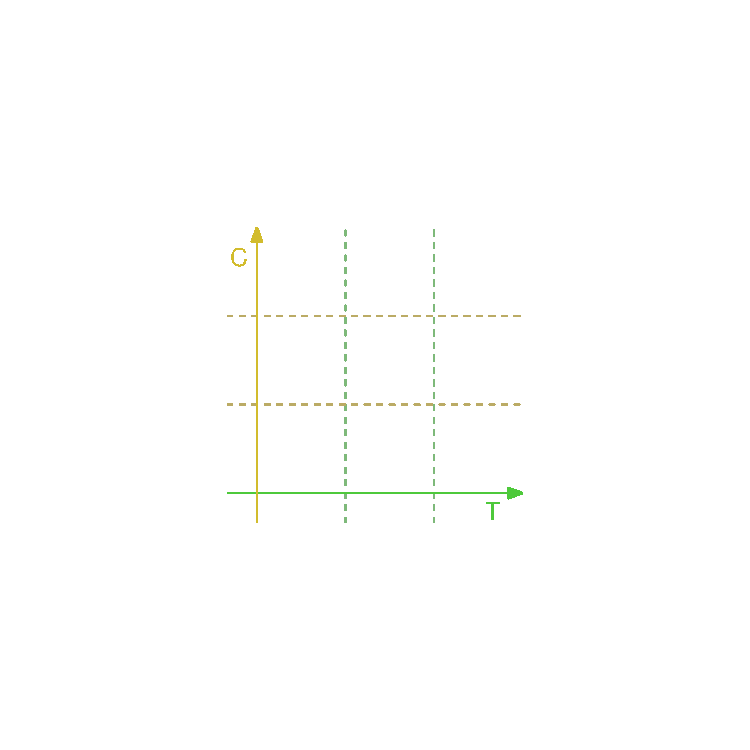
\includegraphics[width = \linewidth]{Figures/JonasTable/CT.pdf} &
  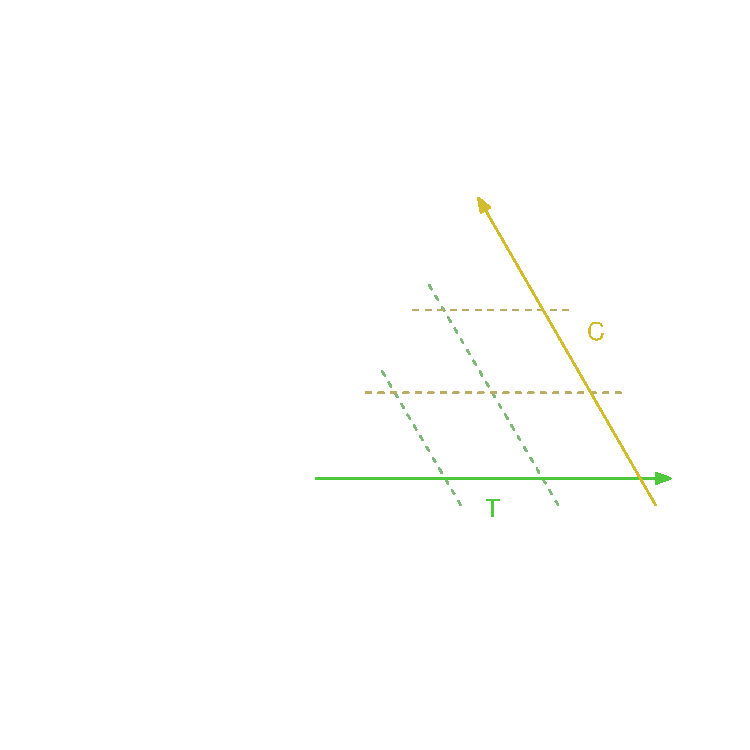
\includegraphics[width = \linewidth]{Figures/JonasTable/CT_iso.pdf}  \\
  \midrule
  %%%% TA
  $$\begin{aligned}
    &TA(L) \\
    &L = T + A
  \end{aligned}$$ &
  The time already lived and the time still left sum up to the total lifespan. &
  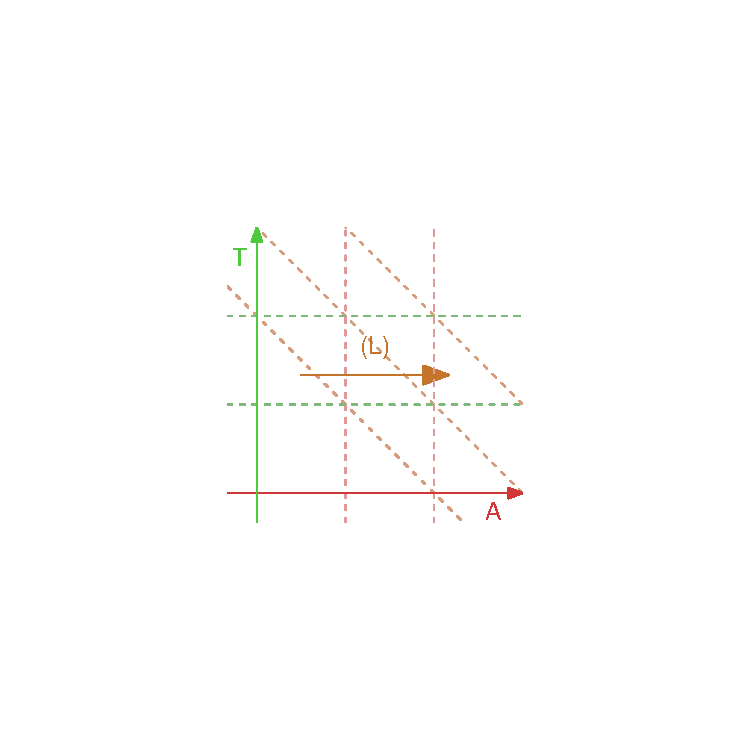
\includegraphics[width = \linewidth]{Figures/JonasTable/TAl.pdf} &
  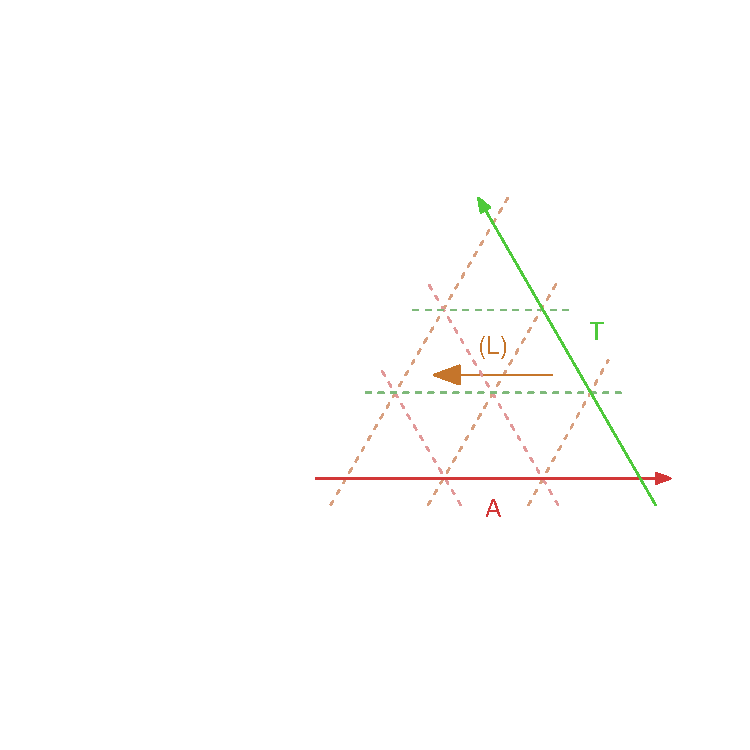
\includegraphics[width = \linewidth]{Figures/JonasTable/TAl_iso.pdf}  \\
  \midrule
  %%%% AD
  $AD(-)$ &
  The $AD$ plane is \emph{non-informative}. No additional dimensions can be derived knowing just death cohort and age. &
  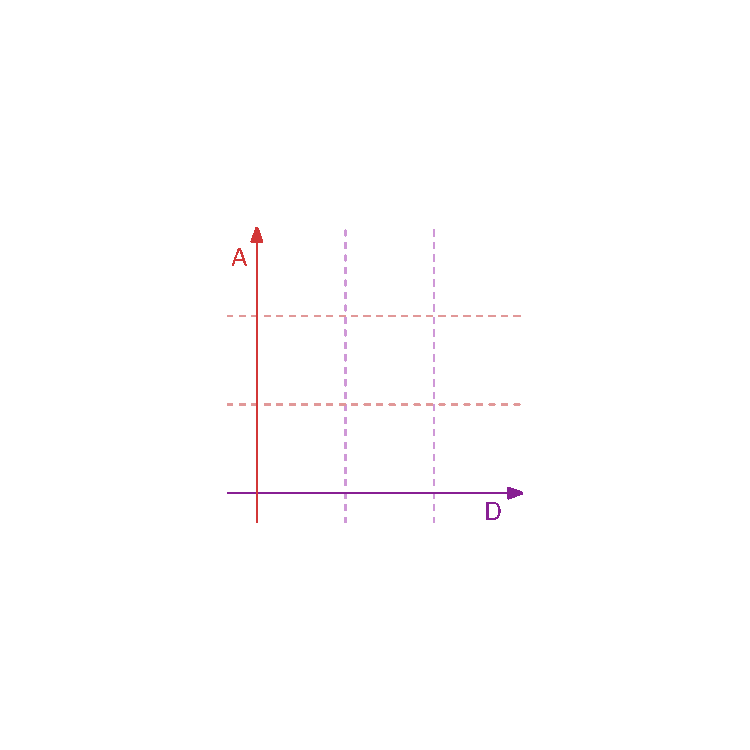
\includegraphics[width = \linewidth]{Figures/JonasTable/AD.pdf} &
  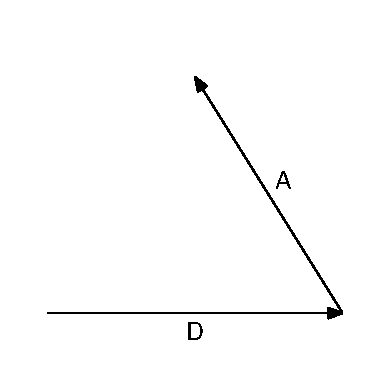
\includegraphics[width = \linewidth]{Figures/JonasTable/AD_iso.pdf}  \\
  \midrule
  %%%% LC
  $$\begin{aligned}
    &LC(D) \\
    &D = C + L
  \end{aligned}$$ &
  {\`A}ngels was born in 1940 (C) and she lived to be 64 (L), implying an
  untimely death in 2004 (D).
  & 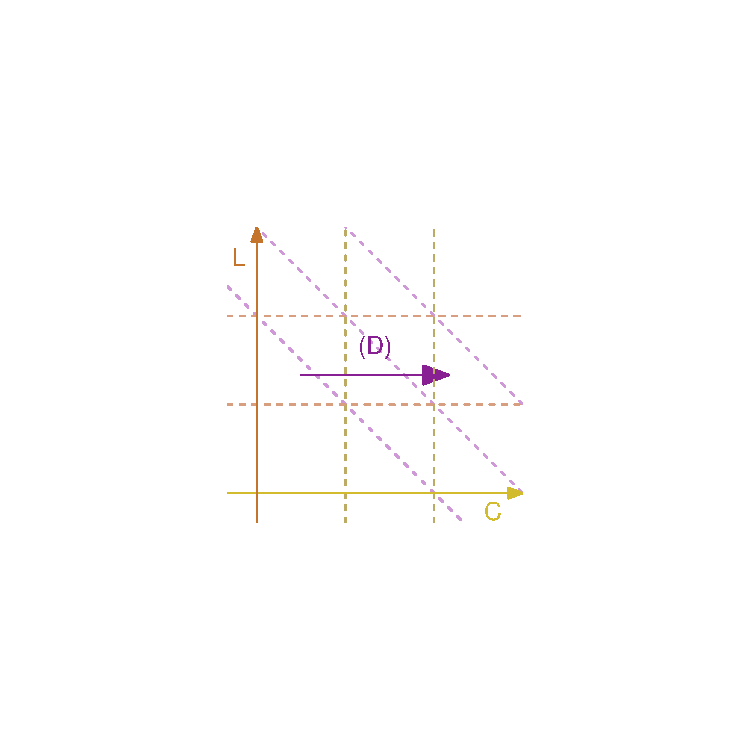
\includegraphics[width = \linewidth]{Figures/JonasTable/LCd.pdf} &
  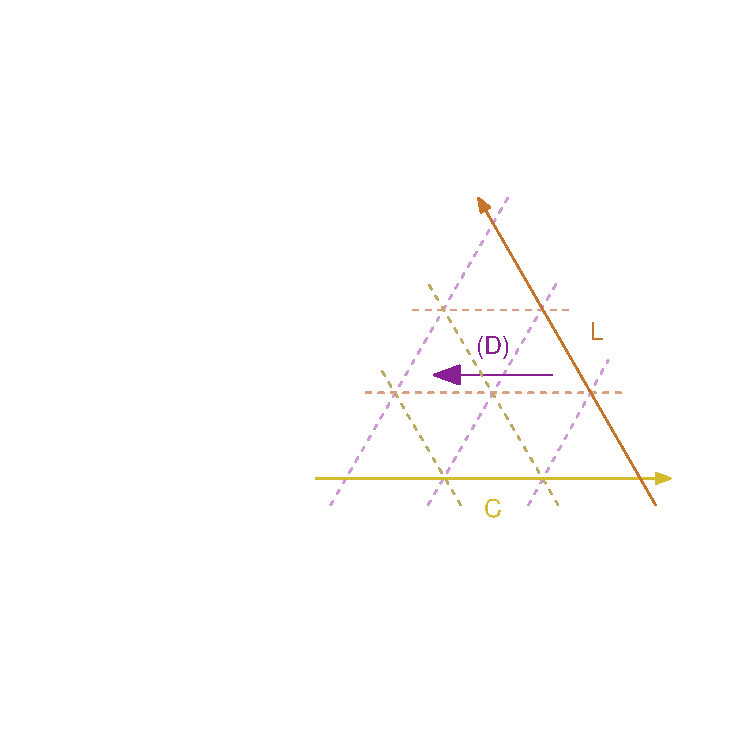
\includegraphics[width = \linewidth]{Figures/JonasTable/LCd_iso.pdf}  \\
  \midrule
  %%%% TP
  $TP(-)$ &
  The $TP$ plane is \emph{non-informative}. No additional dimensions can be derived knowing just thanatological age and period. &
  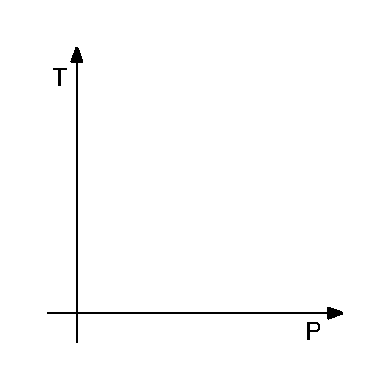
\includegraphics[width = \linewidth]{Figures/JonasTable/TP.pdf} &
  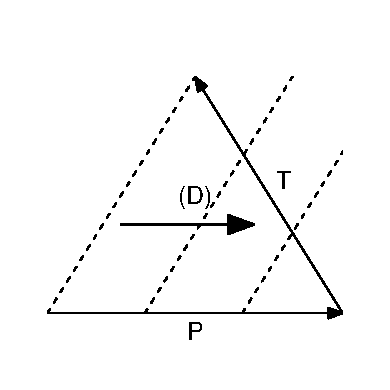
\includegraphics[width = \linewidth]{Figures/JonasTable/TP_iso.pdf}  \\
  \bottomrule
  \end{longtable}
\end{center}



\section*{The triad identities}
Visualizations of data structured by any dyad of time measures mapped onto a
temporal plane from one of the triad identities are inherently richer in
information than juxtapositions of uninformative dyads. There is no reason not
to explore all possible dyadic juxtapositions, but the triad identities have more
apparent meaning, even in the absence of data, due to the underlying
relationship between measures. In the present section, we therefore lay out the
four primary diagrams that belong to the triad identities. This paper contains
no such data visualizations, but it serves as a basis for designing some. Here
we describe the underlying temporal planes of the triad identities.

For the case of each identity,
there is a fundamental question of how to map the constituent coordinates to a
cartesian temporal plane. Typically one forces parity between time units within
a specified dyad, and maps one element directly to $x$ and the second element
directly to $y$, resulting in a 90$^\circ$ angle between the $x$ axis and $y$
axis. In this case the convention is to force a unity aspect ratio
between the $x$ and $y$ axes, such that the derived measure is then
\textit{accidentally} present in a 45$^\circ$ ascending or descending angle,
depending on the dyad and axis orientation. Another possible mapping is to take
the complete triad and translate to an $(x,y)$ coordinate so as to create
60$^\circ$ angles between the three measures. This second mapping is primarily done in order to ensure that the spatial mapping is in equal units for the
three measures, and we therefore refer to it as the isotropic mapping.
The isotropic mapping is comparable to using a ternary coordinate system, which we
do not discuss.

\FloatBarrier
\subsection*{APC}%\tgh{APC}}
The so-called Lexis diagram has long been used in demography as a conceptual
tool for structuring data, observations, and rate estimation, as inspiration for work
on statistical identification, and as the coordinate basis of contemporary
Lexis-surfaces.
Since the Lexis diagram could have been named for others
\citep{vandeschrick2001lexis,keiding2011age}, and since we compare with other
temporal configurations, let us refer to it as the APC diagram, as seen in
Figures~\ref{fig:APCrt} and~\ref{fig:APCeq}. 

\begin{figure} 
\caption{An APC diagram in two projections.}
\label{fig:APC}
\centering
\begin{subfigure}{1.1\textwidth}
\caption{Right angles}
\vspace{-6em}
\label{fig:APCrt}
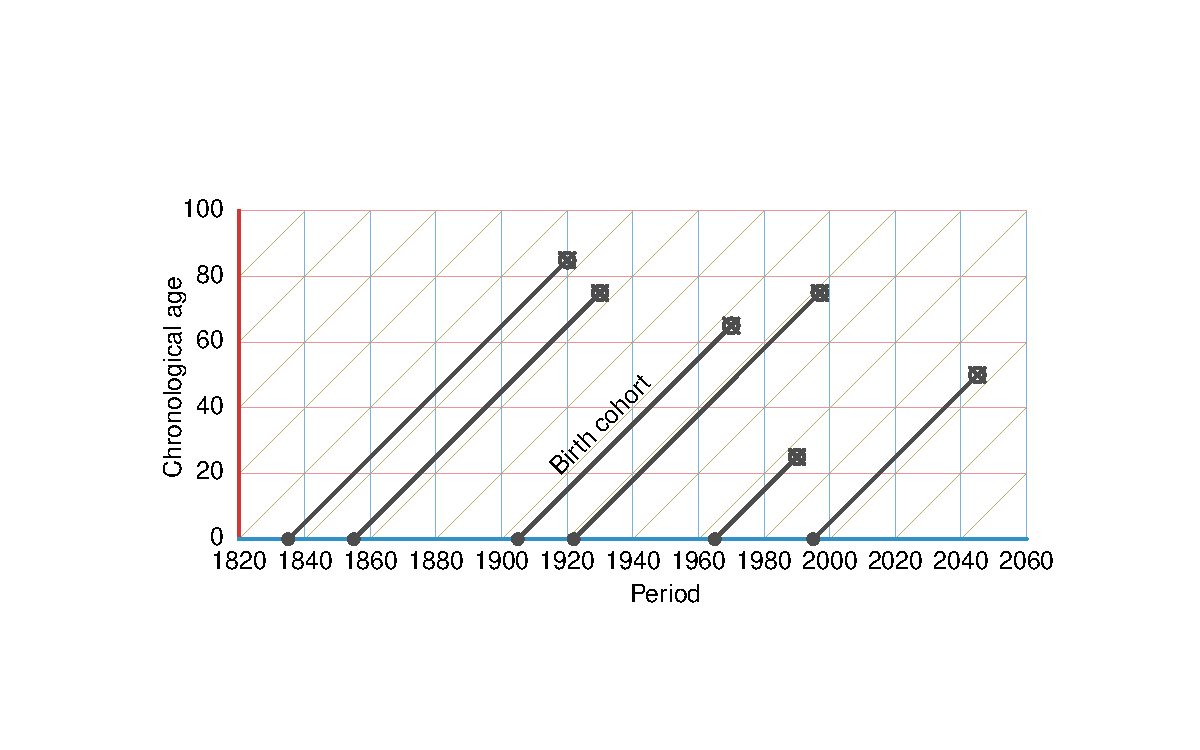
\includegraphics[scale=0.6]{Figures/APCrt.pdf}
\end{subfigure}
\\\vspace{-2em}
\begin{subfigure}{1.1\textwidth}
\caption{All 60$^\circ$ angles}
\vspace{-6em}
\label{fig:APCeq}
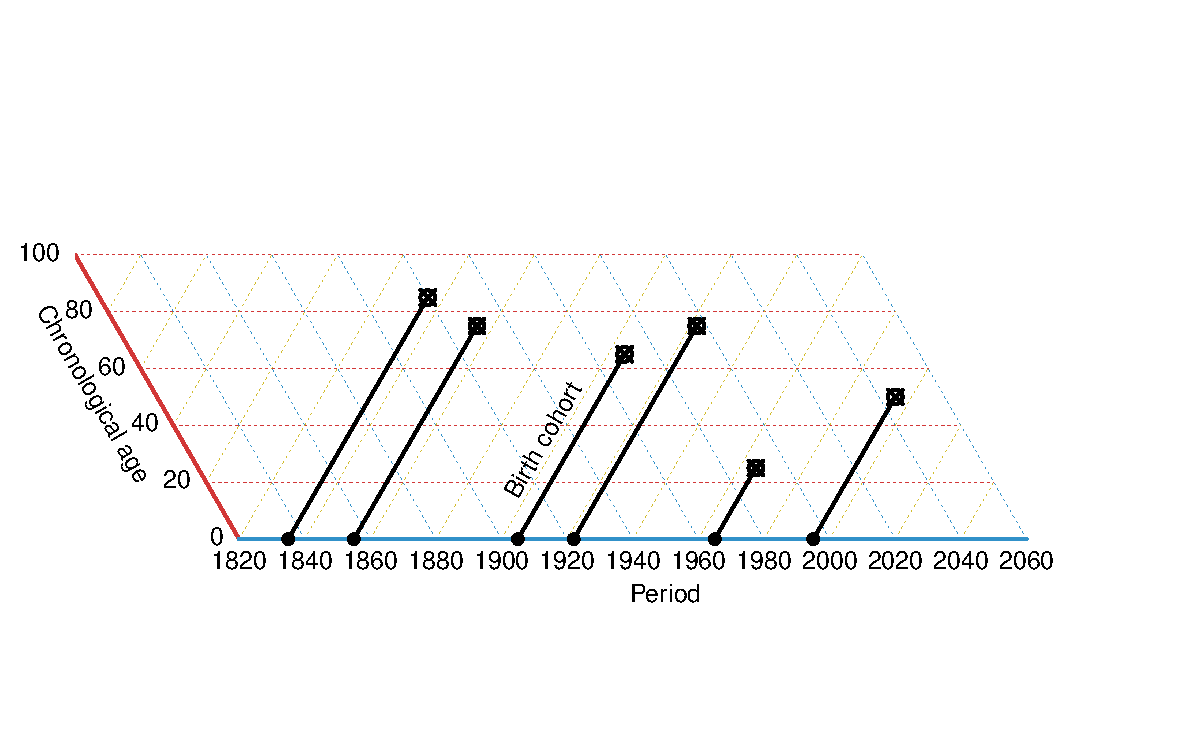
\includegraphics[scale=0.6]{Figures/APCeq.pdf}
\end{subfigure}
\end{figure}

The APC diagram in Figure~\ref{fig:APCrt} represents years lived on the y axis,
calendar years on the x axis, and birth cohorts as the right-ascending
diagonals. This is the most common of several possible configurations
of the APC dimensions. Individual lifelines are aligned in the birth cohort
direction, starting with birth (filled circle) at chronological age zero, and death
(circled x). Any APC surface can be interpreted along each of these
three dimensions of temporal structure. 

It has long been noted \citep{zeuner1869abhandlungen, perozzo1880della} that the
birth cohort dimension, as represented in Figure~\ref{fig:APCrt}, is relatively
longer than either the age or years axes. If a right angle and unity aspect
ratio is forced between any two of the APC dimensions, the third dimension is always be
stretched by $\sqrt{2}$, or 41\% longer. Another long-standing, but less
common variant, is to treat the derived direction (in this case birth cohorts)
as a redundant third axis, and forcing parity between the units of A, P, and C, as in
Figure~\ref{fig:APCeq}. We refer to the second variety as the isotropic APC
diagram, or an equilateral APC diagram. The primary justification for isotropic
temporal planes comes from a data visualization perspective, where it is
supposed that the viewer's ability to compare slopes is hindered if the axes are
not on the same scale. This property will be explored more in a future paper.


\FloatBarrier

\subsection*{TPD}%\tgh{TPD}}
(section in progress, will contain 2 figures, like APC)
*add TPD reference to Villavicencio/Riffe paper under review
Thanatological age (T), period (P) and death cohort (D) form a coordinate system
best imagined as the inverse of APC. One may take the same lifelines from
Figure~\ref{fig:APC} and realign them in descending fashion to create the
diagram in Figure~\ref{fig:TPD}.

\begin{figure} 
\caption{A TPD diagram in two projections.}
\label{fig:TPD}
\centering
\begin{subfigure}{1.1\textwidth}
\caption{Right angles}
\vspace{-6em}
\label{fig:TPDrt}
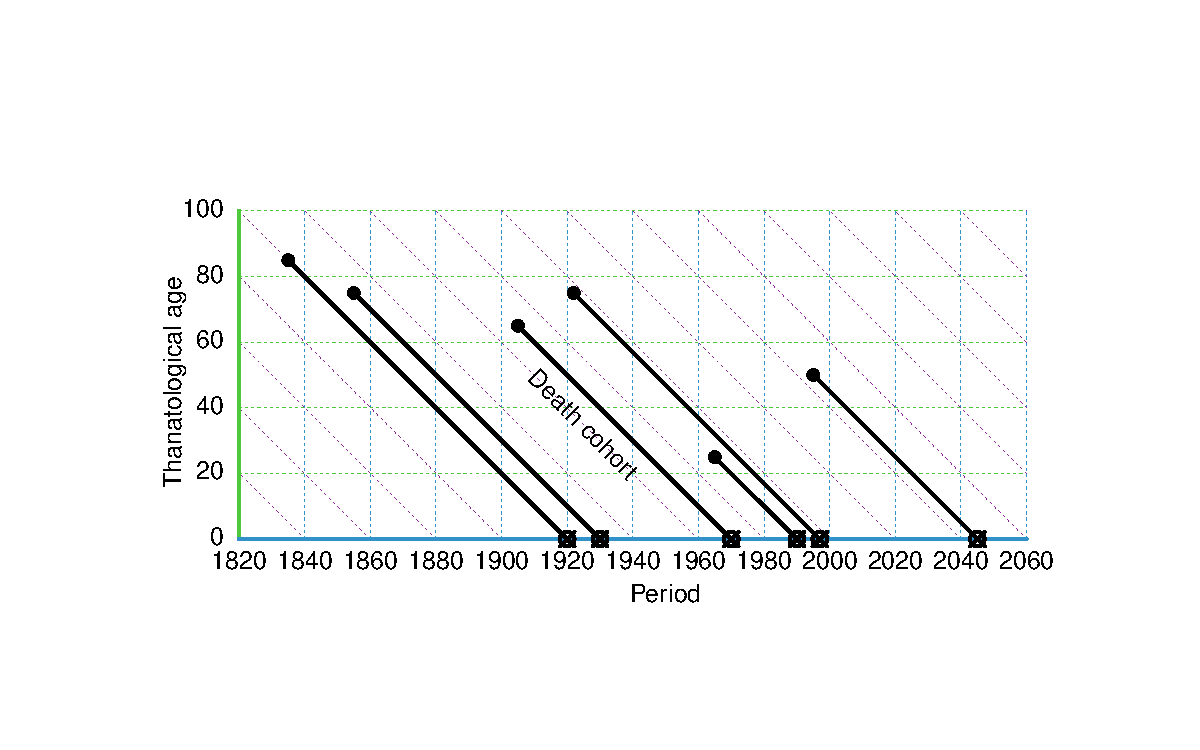
\includegraphics[scale=0.6]{Figures/TPDrt.pdf}
\end{subfigure}
\\\vspace{-2em}
\begin{subfigure}{1.1\textwidth}
\caption{All 60$^\circ$ angles}
\vspace{-6em}
\label{fig:TPDeq}
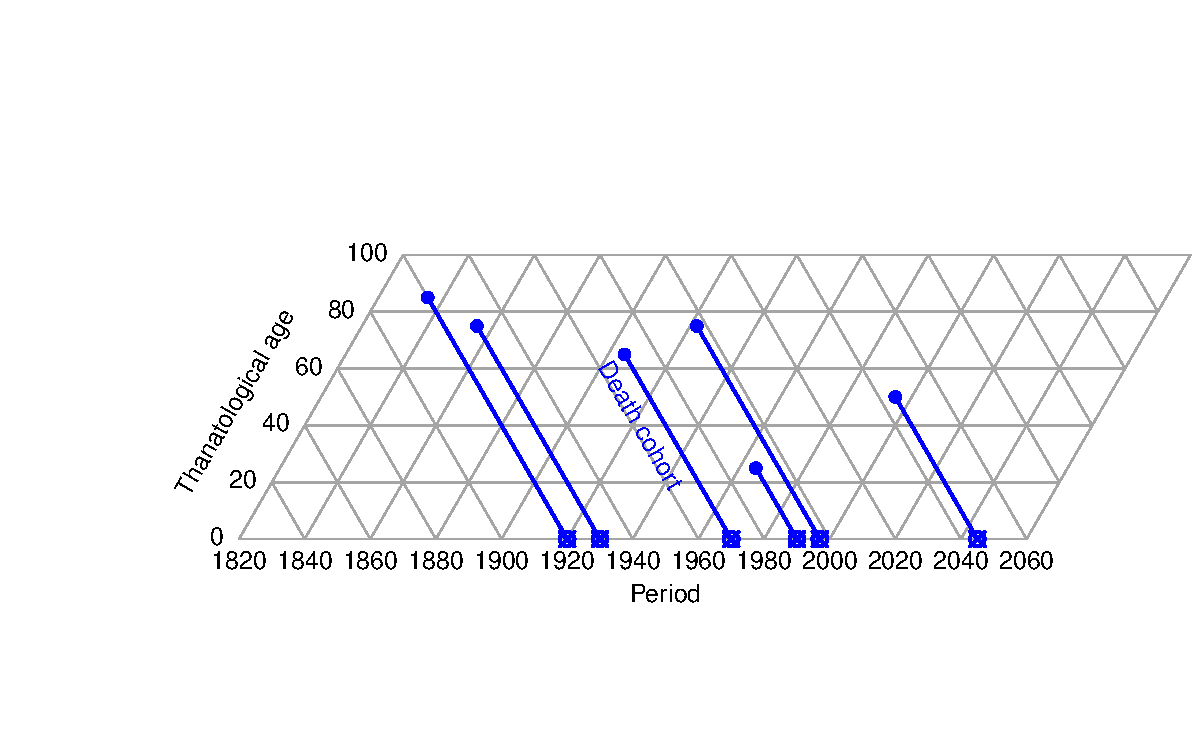
\includegraphics[scale=0.6]{Figures/TPDeq.pdf}
\end{subfigure}
\end{figure} 

\FloatBarrier
\subsection*{ATL}%\tgh{ATL}}
(section in progress, will contain 2 figures, like APC)
*add reference to Riffe, Chung, Spijker, MacInnes (although that ATL was a
cross-section and not a compression) 
The second plane is ATL, a valid coordinate
system for processes that vary over the lifecourse, but not over time (P). Since the
lifecourse belongs to the cohort perspective, it is best to think of the ATL
plane as belonging to some particular birth cohort. Alternatively, an ATL
triangle may be taken as a cross-section along through the period dimension, a
sort of synthetic ATL plane.

\subsection*{CDL}%\tgh{CDL}}
(section in progress, will contain 2 figures, like APC)
* I've not thought much about this one, but it completes the tetrahedron :-P

\section*{A tetrahedron relates the six time indices.}
Each of the four above-mentioned triad identities may be thought of as a
two-dimensional plane fully defined by any two of its three constituent time
indices.
In this case, we may imagine the third ``lacking'' dimension as providing
depth, for the sake of a mental image.
Having a non-redundant third dimension implies a multitude of parallel planes
for the given identity, each plane belonging to a unique value of the third time dimension. Any of the
identities can be extended in this way to fill a space. A space derived by
extending any of the triad identies into its lacking dimension implies each of the
other triad identities, making a total of six time indices. In essence, the
four triad identities may be thought of as \sout{parallel to }the four faces of a
tetrahedron. \sout{In this case, the four ``lacking'' dimensions may be assigned to
the four vertices of the tetrahedron, and the six demographic time indices match
to the six edges of the tetrahedron.} \textbf{If an additional time-index dimension is added to each face (triad identity), the six demographic time indices can be derived, matching the six edges of the tetrahedron.} This three-dimensional construct
unifies the six indices of demographic time, and is the subject of this paper.

Let us first more rigorously define the previously-mentioned tetrahedron.
Luckily, the edges and vertices of a tetrahedron are easily rendered in a
two-dimensional graph, as seen in Figure~\ref{fig:tet}, with vertices labeled
in red and the six time indices labeled as blue edges.\footnote{The same graph
could be composed in four basic ways, depending on which \sout{vertex is in the
middle} \textbf{triad-identity face in in the bottom}. These are given in an appendix.} The reader may also imagine this graph
as a transparent 3d object, in which case the four faces become aparent. There are two intuitive ways to imagine the graph as 3d, either the vertex 4 is on top, and we gaze from a bird's-eye-view, or the
vertex 4 is in the back, behind the other three vertices. Assume we
gaze from the top, for the sake of description. 

\begin{figure}[h!]
\centering
\caption{Graph of tetrahedron, with edges labeled by the six demographic time
indices.}
\label{fig:tet}
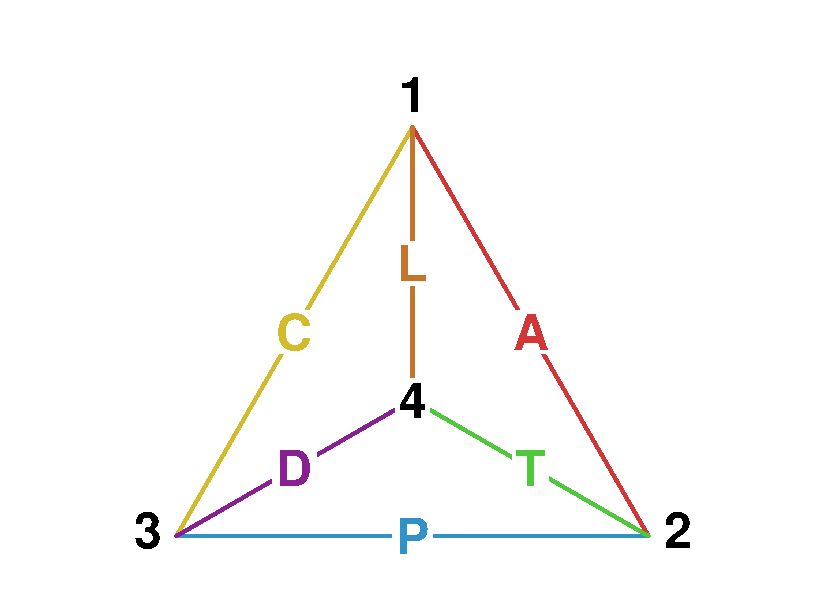
\includegraphics[scale=1]{Figures/TetraHedronVerticesEdges.pdf}
\end{figure}

\subsection*{Information criteria to derive the tetrahedron.}
The edges APC at the base define the much-studied APC plane. If the only
information we have is chronological age, period, and birth cohort (or just two
of these), then we have no access to the vertex 4. Each of the faces of the
tetrahedron has this quality. The South face TDP has no access to 1.
The Northeast face, ATL has no connection to 3, and the Northwest face
CDL lacks a connection to 2. The triads that make up the faces of
the tetrahedron are stuck in ``flatland''. However, there are $\binom{6}{3}=20$ ways to choose three time indices out of six, and the four
above-named triads are the only ones that will not yield the full 3d
space and imply the other three. The sixteen other combinations of three indices will recreate the full tetradhedron (hexad identity).


% PV: I suggest to replace the following paragraph, or at least to introduce
% this geometrical perspective somewhere in the text

%   TR: OK, I've commented it out. The removed paragraph sounds more like advice
%       on how to manually find all 20-16-12 triads without too much mental
%       labor. Maybe worth an appendix?
% TR: the vector description is probably more rigorous, so let's go with it.
%     We'll put some effort later into making it understandable for avg
%     demographers.

%\sout{For example, say we are at vertex \vt{1}, and we therefore have
%information on year of birth C, completed lifespan L, and
%chronological age A (see Figure~\ref{fig:tet4vert1}). Clearly, A and
%C imply P ($C+A=P$).
%A and L imply T ($L-A=T$). Finally, C and
%L imply D ($C+L=D$), and we have the full hexad
%identity. In the tetrahedron graph, we have three edges that connect to the
%four vertices. This is the essential property of a fully informed triad.
%It is easily verified that each vertex has this property.
%However, there are twelve other sets of three that also have this property. To
% locate these ``hidden'' triads, first note that each index has an
%opposite index, with which it shares no information. These pairs are
%A-D, L-P, and C-T, and can be found in Figure~\ref{fig:tet} as
%the three sets of perpendicular edges. Each of these pairs can be completed
% into a `fully-informed'' triad by the addition of any of the other four indices
%(thereby connecting the edges). Doing so for each of the opposite pairs will
%yield the remaining twelve triads.}

A geometrical analogy is pertinent at this point. Any pair of intersecting edges
of the tetrahedron may be interpreted as two vectors $\vec{u}$ and $\vec{v}$
that determine a 2-dimensional plane in a 3-dimensional
space.\footnote{A 2d plane in a 3d space is determined by two linearly independent
vectors (with different direction) and a point, but the inclusion of a point is not
necessary for the intuitive analogy that we describe here.} Therefore, any third
vector $\vec{w}$ of that plane can be expressed as a linear combination of
$\vec{u}$ and $\vec{v}$ (formally, $\vec{w}=\alpha\vec{u}+\beta\vec{v}$ for some $\alpha, \beta \in \mathbb{R}$), which is usually
referred as saying that $\vec{w}$ is linearly dependent on $\vec{u}$ and $\vec{v}$. A similar property can be derived from the information contained in the tetrahedron: Say we have information on year of birth $C$ and period $P$. Clearly, $C$ and $P$ are sufficient to determine the chronological age $A$, given that  $A=P-C$. That is, $A$ is a linear combination of $C$ and $P$ and it ``depends'' on them because they all belong to the same $APC$ plane (see Figure~\ref{fig:tet4vert1}). Analogously, $P=C+A$ ``depends'' on $C$ and $A$, and $C=P-A$ ``depends'' on $P$ and $A$. It can be easily verified that any pair of intersecting edges have the same propriety: The third edge located in the same face of the tetrahedron can be determined by the first two by a simple linear relationship.

% code given in R/TetraCombos.R, lines 70-95
% PV: already created the new figure
\begin{figure}[h!]
\centering
\caption{Graph of tetrahedron, edges eminating from vertice \vt{1} highlighted.}
\label{fig:tet4vert1}
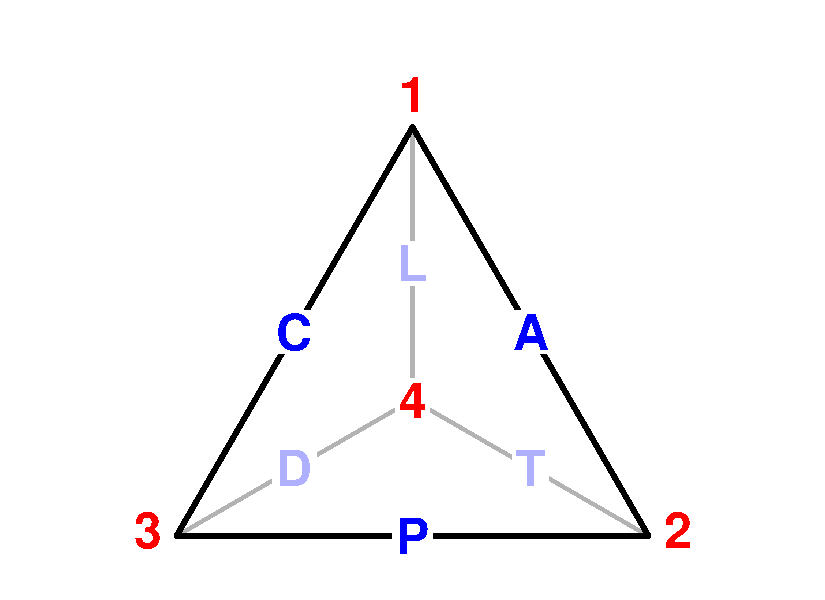
\includegraphics[scale=1]{Figures/tet4vert1New.pdf}
\end{figure}
\noindent 

Once a 2d-plane is defined, an additional vector may be sufficient to cover the whole 3d-space. Nonetheless, this third vector needs to be linearly independent of any pair of vectors of that 2d plane---that is, it cannot be expressed as a linear combination of any two vectors on that plane. Again, an analogous propriety can be observed in the tetrahedron: Say we only have information about the indices of the $APC$ plain; $A$, $C$ and $P$ are not sufficient to determine a thanatological age $T$, death cohort $D$, or lifespan $L$ (the three indices that do not belong to the $APC$ plane). So, $T$, $D$ and $L$ are ``independent'' of the overall information that can be extracted from the $APC$ plane. However, if two of the three constituent time indices of the $APC$ plane are known (the third one would be
unnecessary as it could be derived from the other two), the additional
information provided by any of the three ``independent'' indices $T$, $D$ or
$L$ would be sufficient to cover the whole tetrahedron. For example, suppose we
have information about thanatological age $T$ in addition to $C$ and $P$, then
$A=P-C$, $D=P+T$ and $L=T+A=T+P-C$. 

Hence, as with vectors in a 3d space, any
triad of indices that are independent of each other---that is, none of them can
be expressed as the sum or the difference of the other two---generates a full
hexad identity or, using an analogous terminology, covers the whole ``space'' of
demographic indices presented in this paper. Graphically, this is equivalent to
choosing any combination of three indices that do not belong to the same face
of the tetrahedron, i.e. that they do not form one of the four triad identities represented in Table~\ref{tab:triadids}.

\begin{table}[h]
\centering
\caption{The four triad identities on the tetrahedron (same orientation)}
\label{tab:triadids}
\begin{tabular}{cccc}
APC & TPD & ATL & CDL\\
\tg{APC} & \tg{TPD} & \tg{ATL} & \tg{CDL}
\end{tabular}
\end{table}

\sout{A like-organized table for the four triad identities simply highlights each of
the four faces of the tetrahedron, as seen in Table~\ref{tab:triadids}. When
graphed in this way, the vertex lacking a connection becomes clearer.} \textbf{When graphed in this way, it is clearer that every triad identity surface lacks a connection to the opposite vertex of the tetrahedron.} We
therefore say that each of the triad identities is incomplete. Table~\ref{tab:set3} gives the full set of sixteen index-triads that are
complete in this sense. It can be verified that each of these
triads implies the full hexad identity. \sout{This property is comparable to the
reducibility characteristic of triad identities. For example, for the APC
identity, the list of dyads that give full information is shorter:
AC, AP, PC. The triads in Table~\ref{tab:set3} give analogous
information for the APCTDL identity.
It may be further stated that no dyad of indices will give the hexad identity,
and any quad (or greater) of indices will yield the hexad identity. Any index
complemented by any index other than its opposite will imply one of
the triad identities.}

\textbf{Note that any pair of time indices generate one of the four triad identities in Table~\ref{tab:triadids}, but no dyad will generate the hexad identity given that a third ``independent'' time dimension is necessary. 
Similarly, any quad of indices is sufficient to complete the hexad identity, as at least one of them will not belong to the same face of the tetrahedron, but a triad may be sufficient if they 
do not all belong to the same plane forming a triad identity.}

\begin{table}[h]
\centering
\caption{All sets of three indices that imply the full six indices, graphed
given the previous orientation of the tetrahedron.}
\label{tab:set3}
\begin{tabular}{cccc}
ACD & ACL & ACT & ADL\\
\tg{ACD} & \tg{ACL} & \tg{ACT} & \tg{ADL}\\
ADP & ADT & ALP & APT\\
\tg{ADP} & \tg{ADT} & \tg{ALP} & \tg{APT}\\
CDP & CDT & CLP & CLT\\
\tg{CDP} & \tg{CDT} & \tg{CLP} & \tg{CLT}\\
CPT & DLP & DLT & LPT\\
\tg{CPT} & \tg{DLP} & \tg{DLT} & \tg{LPT}
\end{tabular}
\end{table}

\subsection*{The extension of time axes.}
We have said that planes defined by the four triad identities are parallel to
the faces of the the above-described tetrahedron. In imagining this three-dimensional
relationship, we are no longer confined to the extent of the tetrahedron that
we have used thus far for orientation. Instead each of its edges extends a
certain distance in either direction.
It may therefore help to first consider the extension of each axis (or index).
Some indices have a lower bound of zero and an upper bound set by the maximum
length of life, $\omega$, while others are boundless. A, T, and L
are clearly in the range $[0,\omega]$.\footnote{It's best to imagine some number like 122.45 years, for $\omega$, rather than infinity. This is the longevity record at the time of this writing. Jeanne L. Calment would have had
$T=122.45$ at birth, $A = 122.45$ at death, and $L=122.45$ for
her entire life.} P, C, and D are bounded only by the inception and extinction of
our species, but may be thought of as boundless for practicality, or benchmarked
to our earliest and most recent observations for even more
practicality.\footnote{We explain the choice of the word ``benchmarked''. Say
we have a data series that runs from 1751 to 2011, and an upper age
interval of $110+$. Then we could say that P is in the range $[1751,2011]$,
but by another reading, P must range from at least as early as the earliest
C and until at least as late as the latest D. Someone dying at 110 in 1751
had a C of 1640, and an infant born in 2011 that is destined to live to 110
will die in 2121. In this case a P that \textit{contains} the observed
population will extend well before and after the observed data series, even
moreso if we take into account that $\omega > 110$.} As an abstraction,
however, the dimension of calendar time in this model is infinite. Of the four
triad identities, only one lacks an unbounded dimension, the ATL. Adding
the absent dimension to ATL therefore makes its 3d extension boundless. In
this way, we may imagine a prism-like construct, where A, T, and L, compose
the faces of a triangular cross-section of said prism, which extends infinitely ``through'' the triangle.
We can think of the ATL triangle passing through time, extending the population
forward to infinity. In this case, the ATL triangle may take either the period
or cohort perspective, and this will be explained later. 

There are also
numerous ways that this three dimensional construct can be proportioned, of
which we present two in this paper. The first stems from the respect given to
right angles in the most common representation of the Lexis diagram. For this reason, it will likely be
the most intuitive rendition of the model, and it will be presented first. The
second version presented is isotropic with respect to time units in each of the
six temporal indices. In this case, the four tripartite identities are based on
equilateral triangles between their three constituent indices, and the four
planes are joined together such that each is parallel to a face from the regular
tetrahedron, a construct known in geometry as an octahedral-tetrahedral
honeycomb.

\section*{Intersecting planes}

The APC, TPD, ATL, and CDL planes can be conceived of as
\textit{compressions} of this 3d space, or as cross-sections of the 3d space. To
compress the space in this sense is to ignore the missing dimension,
whereas a cross-section sets a given triad identity against a particular
position of the absent dimension. APC has thus far always been treated as a
compression, and myriad such uses and examples are familiar to demographers.
A compressed TPD diagram has thus far only appeared in \citet{pancho2015}
as an aid in \sout{explaining a mathematical proof}\textbf{proving the symmetries between chronological and thanatological age in stationary populations}, and a cross-sectional one has
never appeared.
Cross-sectional ATL diagram and surfaces have thus far only appeared in
\citet{riffe2015ttd}. This ATL usage was selected for the 1915-1919 birth
cohort, and therefore belongs to the 3d
space,
\raisebox{-.25\height}{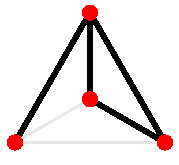
\includegraphics[scale=.15]{Figures/triadtable/ATLC.pdf}}.
We have been unable to located an example in the literature of a compressed
ATL diagram, but it seems likely one will have arisen in the field of
biology, albeit with no relation to the present discourse. We suppose
that CDL diagrams of any kind are yet-unknown.


\section*{APCT}
*section ignored for the present: plan for a table with different distilled 3d
views of the contruct, probably vector snapshots of an RGL model. Probably each
will be centered on a single tetrahedron, with sides labeled, and one face of
it (triad identity) will be highlighted and extended, and given depth). Each
face will be seen from 2 angles, and also for the right and isotropic
projections. use lighting, etc, to give depth. Need to work hard on this, but no
rush.

*Again, the following stuff is from the original proposal and will be completely
superceded, though tidbits still hold.

 We
propose a geometric identity that unifies all such temporal notions into a single (simple) spatial relationship that serves as an omnibus conceptual aid to demographers, much as the Lexis diagram does for APC relationships. The full result is a three dimensional space that can be disected by any of four different planes, each of which is parallel to the faces of a regular tetrahedron (see
Figure~\ref{fig:APCT} for a first mock-up of the model).
Each dissecting plane relates three indices of demographic time in proportion to one
another (1:1:1 ternary aspect ratio). The complete space can be described in
geometry nomenclature as the tetrahedral-octahedral honeycomb, which is a kind of space-filling tessellation.\footnote{Constructs following
this geometry exist both in nature and in man-made structures.} 
One of these planes is the familar Lexis plane (horizontal planes in
Figure~\ref{fig:APCT}, and the other three will be new surprises for
demographers. This three dimensional space is not only useful for the sake of formalizing observed temporal relationships, but also for encolosing
demographic time in the past and future (e.g., before the first census and after
the most recent census). 

\begin{figure}[!h]
\centering
\caption[cap]{A mock-up example of the unified model of demographic
time.\footnotemark}
\label{fig:APCT}
	\includegraphics[bb=0 0 3264 2448, width=.8\textwidth]{Figures/PhysicalModel.jpg}
\end{figure}
\footnotetext{This and other figures to be replaced with vector graphics, although
	I may bring this model to the presentation, since it helps explain concepts.}

A property of the geometry that we propose is that
the time units in every direction (with respect to each index) are proportional. The Lexis
diagram based on right angles and $45^\circ$ birth cohort lines does not have
this property, whereas Lexis diagrams and surfaces based on equilateral
triangles, such as some early proposals \citep[inter
alia, ][]{lexis1875einleitung, lewin1876rapport}, the masterful stereogram of
\citet{perozzo1880della}, or the more recent APC diagram
of \citet{ryder1980cohort}, do have this property. The disecting planes of the
model I propose are likewise composed of equilateral triangles. In Lexis
nomenclature, the 3d projections of an AP square, and AC or PC
parallelograms are all congruent shapes known as regular trigonal trapezohedra
(RTT). The orientation
of a given RTT uniquely defines the Lexis shape in question. Similar constructs
exist in the other time dimensions, and these will also be described. 
\FloatBarrier

\begin{appendices}
\section{Variants of tetrahedron graph}
The graph depicted in Figure~\ref{fig:tet} could be drawn with any of the
four vertices in the middle of the triangle (as well as other inversions
and rotations).
These would all serve equally well to present the same aspects of the model, and
we have no insight as to whether one of these renditions is more or less
intuitive. Figure~\ref{fig:app:tet} provides four perspectives on the
tetrahedron, for the case that this aids in understanding. The reader may make a
paper tetrahedron, with labeled edges and vertices to be convinced that
these are identical graphs.
\begin{figure*}
        \centering
        \caption{Some variants of the graph of the APCTDL tetrahedron.} 
         \label{fig:app:tet}
        \begin{subfigure}[b]{0.475\textwidth}
            \centering
            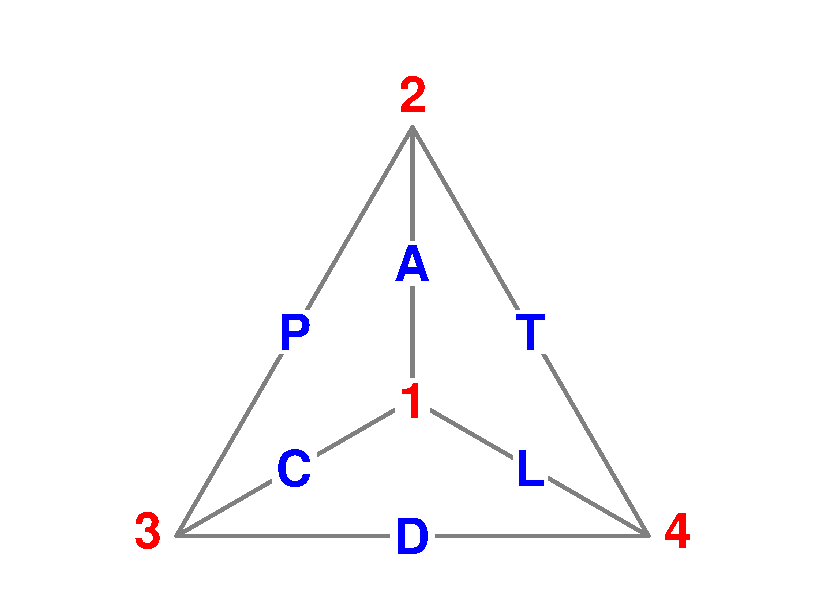
\includegraphics[width=\textwidth]{Figures/Tetra1.pdf}
           \caption{\small Vertex \vt{1} in middle. APC Northwest.}
            \label{fig:tet1}
        \end{subfigure}
        \hfill
        \begin{subfigure}[b]{0.475\textwidth}  
            \centering 
            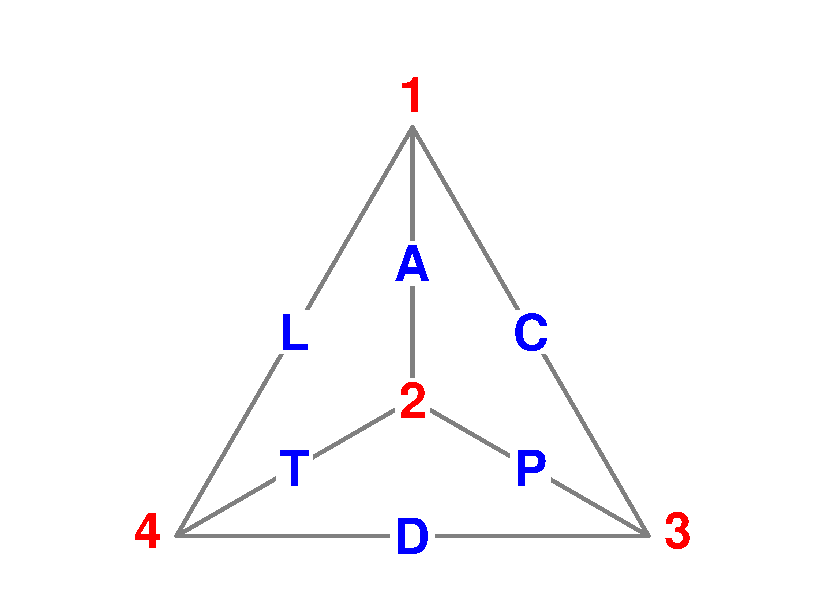
\includegraphics[width=\textwidth]{Figures/Tetra2.pdf}
           \caption{\small Vertex \vt{2} in middle. APC Northeast.}
            \label{fig:tet2}
        \end{subfigure}
        \vskip\baselineskip
        \begin{subfigure}[b]{0.475\textwidth}   
            \centering 
            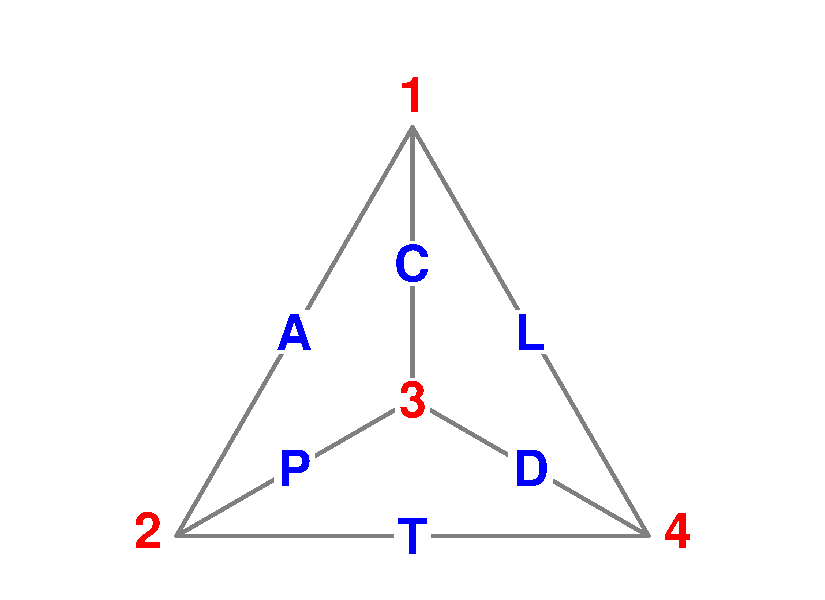
\includegraphics[width=\textwidth]{Figures/Tetra3.pdf}
           \caption{\small Vertex \vt{3} in middle. APC Northwest.}
            \label{fig:tet3}
        \end{subfigure}
        \quad
        \begin{subfigure}[b]{0.475\textwidth}   
            \centering 
            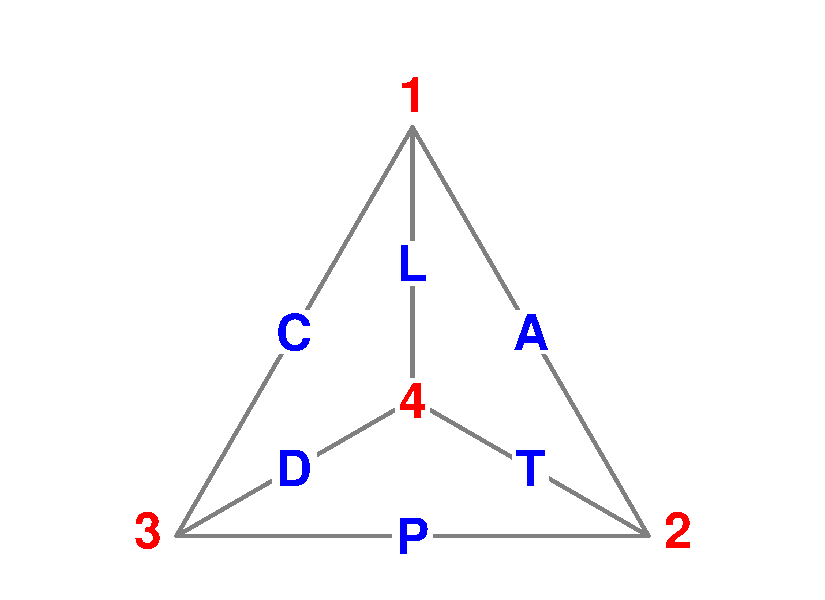
\includegraphics[width=\textwidth]{Figures/Tetra4.pdf}
            \caption{\small Vertex \vt{4} in middle, as in
            Figure~\ref{fig:tet}. APC base.}
            \label{fig:tet4}
        \end{subfigure}
    \end{figure*}
\end{appendices}
\FloatBarrier

\bibliographystyle{plainnat}
  \bibliography{references} 



\end{document}